\documentclass{standalone}
\usepackage{tikz}
\usetikzlibrary{patterns, positioning}


\begin{document}
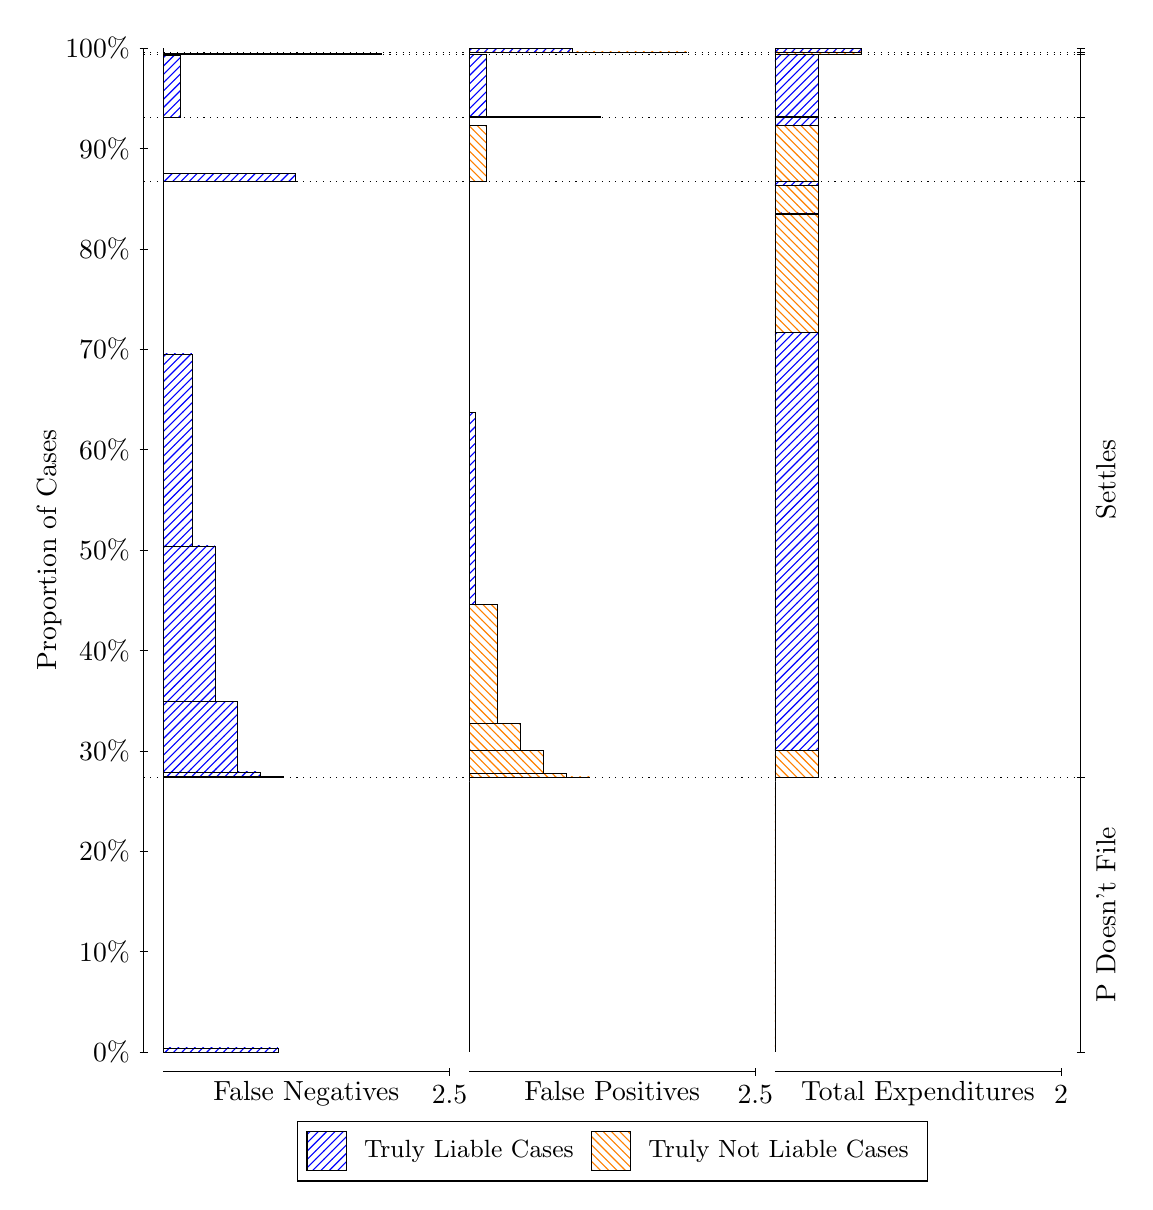
\begin{tikzpicture}
\draw[black, very thin] (1.5,1.75) -- (1.5,14.5);
\node[rotate=90, text=black, anchor=center] at (0.3, 8.125) {Proportion of Cases};
\draw[black, very thin] (1.45,1.75) -- (1.55,1.75);
\node[text=black, anchor=east] at (1.45, 1.75) {0\%};
\draw[black, very thin] (1.45,3.025) -- (1.55,3.025);
\node[text=black, anchor=east] at (1.45, 3.025) {10\%};
\draw[black, very thin] (1.45,4.3) -- (1.55,4.3);
\node[text=black, anchor=east] at (1.45, 4.3) {20\%};
\draw[black, very thin] (1.45,5.575) -- (1.55,5.575);
\node[text=black, anchor=east] at (1.45, 5.575) {30\%};
\draw[black, very thin] (1.45,6.85) -- (1.55,6.85);
\node[text=black, anchor=east] at (1.45, 6.85) {40\%};
\draw[black, very thin] (1.45,8.125) -- (1.55,8.125);
\node[text=black, anchor=east] at (1.45, 8.125) {50\%};
\draw[black, very thin] (1.45,9.4) -- (1.55,9.4);
\node[text=black, anchor=east] at (1.45, 9.4) {60\%};
\draw[black, very thin] (1.45,10.675) -- (1.55,10.675);
\node[text=black, anchor=east] at (1.45, 10.675) {70\%};
\draw[black, very thin] (1.45,11.95) -- (1.55,11.95);
\node[text=black, anchor=east] at (1.45, 11.95) {80\%};
\draw[black, very thin] (1.45,13.225) -- (1.55,13.225);
\node[text=black, anchor=east] at (1.45, 13.225) {90\%};
\draw[black, very thin] (1.45,14.5) -- (1.55,14.5);
\node[text=black, anchor=east] at (1.45, 14.5) {100\%};

\draw[black, very thin] (13.4,1.75) -- (13.4,14.5);
\draw[black, very thin] (13.35,1.75) -- (13.45,1.75);
\node[anchor=west] at (13.35, 1.75) {};
\draw[black, very thin] (13.35,5.2391) -- (13.45,5.2391);
\node[anchor=west] at (13.35, 5.2391) {};
\draw[black, very thin] (13.35,12.807) -- (13.45,12.807);
\node[anchor=west] at (13.35, 12.807) {};
\draw[black, very thin] (13.35,13.617) -- (13.45,13.617);
\node[anchor=west] at (13.35, 13.617) {};
\draw[black, very thin] (13.35,14.423) -- (13.45,14.423);
\node[anchor=west] at (13.35, 14.423) {};
\draw[black, very thin] (13.35,14.448) -- (13.45,14.448);
\node[anchor=west] at (13.35, 14.448) {};
\draw[black, very thin] (13.35,14.5) -- (13.45,14.5);
\node[anchor=west] at (13.35, 14.5) {};

\draw[black, very thin, pattern color=blue, pattern=north east lines] (1.75,1.75) rectangle (3.2033,1.8012);
\draw[black, very thin, pattern color=orange, pattern=north west lines] (1.75,1.8012) rectangle (1.75,5.2391);
\draw[black, very thin, pattern color=blue, pattern=north east lines] (1.75,5.2391) rectangle (3.276,5.2531);
\draw[black, very thin, pattern color=blue, pattern=north east lines] (1.75,5.2531) rectangle (2.9853,5.3069);
\draw[black, very thin, pattern color=blue, pattern=north east lines] (1.75,5.3069) rectangle (2.6947,6.2025);
\draw[black, very thin, pattern color=blue, pattern=north east lines] (1.75,6.2025) rectangle (2.404,8.1761);
\draw[black, very thin, pattern color=blue, pattern=north east lines] (1.75,8.1761) rectangle (2.1133,10.616);
\draw[black, very thin, pattern color=orange, pattern=north west lines] (1.75,10.616) rectangle (1.75,12.807);
\draw[black, very thin, pattern color=blue, pattern=north east lines] (1.75,12.807) rectangle (3.4213,12.906);
\draw[black, very thin, pattern color=orange, pattern=north west lines] (1.75,12.906) rectangle (1.75,13.617);
\draw[black, very thin, pattern color=blue, pattern=north east lines] (1.75,13.617) rectangle (1.968,14.409);
\draw[black, very thin, pattern color=orange, pattern=north west lines] (1.75,14.409) rectangle (1.75,14.423);
\draw[black, very thin, pattern color=blue, pattern=north east lines] (1.75,14.423) rectangle (4.5113,14.43);
\draw[black, very thin, pattern color=orange, pattern=north west lines] (1.75,14.43) rectangle (1.75,14.448);
\draw[black, very thin, pattern color=orange, pattern=north west lines] (1.75,14.448) rectangle (1.75,14.452);
\draw[black, very thin, pattern color=blue, pattern=north east lines] (1.75,14.452) rectangle (1.75,14.5);
\draw[black, very thin, pattern color=orange, pattern=north west lines] (5.6333,1.75) rectangle (5.6333,5.1879);
\draw[black, very thin, pattern color=blue, pattern=north east lines] (5.6333,5.1879) rectangle (5.6333,5.2391);
\draw[black, very thin, pattern color=orange, pattern=north west lines] (5.6333,5.2391) rectangle (7.1593,5.2435);
\draw[black, very thin, pattern color=orange, pattern=north west lines] (5.6333,5.2435) rectangle (6.8687,5.2882);
\draw[black, very thin, pattern color=orange, pattern=north west lines] (5.6333,5.2882) rectangle (6.578,5.5769);
\draw[black, very thin, pattern color=orange, pattern=north west lines] (5.6333,5.5769) rectangle (6.2873,5.9233);
\draw[black, very thin, pattern color=orange, pattern=north west lines] (5.6333,5.9233) rectangle (5.9967,7.4301);
\draw[black, very thin, pattern color=blue, pattern=north east lines] (5.6333,7.4301) rectangle (5.706,9.87);
\draw[black, very thin, pattern color=blue, pattern=north east lines] (5.6333,9.87) rectangle (5.6333,12.807);
\draw[black, very thin, pattern color=orange, pattern=north west lines] (5.6333,12.807) rectangle (5.8513,13.517);
\draw[black, very thin, pattern color=blue, pattern=north east lines] (5.6333,13.517) rectangle (5.6333,13.617);
\draw[black, very thin, pattern color=orange, pattern=north west lines] (5.6333,13.617) rectangle (7.3047,13.63);
\draw[black, very thin, pattern color=blue, pattern=north east lines] (5.6333,13.63) rectangle (5.8513,14.423);
\draw[black, very thin, pattern color=orange, pattern=north west lines] (5.6333,14.423) rectangle (5.6333,14.44);
\draw[black, very thin, pattern color=blue, pattern=north east lines] (5.6333,14.44) rectangle (5.6333,14.448);
\draw[black, very thin, pattern color=orange, pattern=north west lines] (5.6333,14.448) rectangle (8.3947,14.452);
\draw[black, very thin, pattern color=blue, pattern=north east lines] (5.6333,14.452) rectangle (6.9413,14.5);
\draw[black, very thin, pattern color=orange, pattern=north west lines] (9.5167,1.75) rectangle (9.5167,5.1879);
\draw[black, very thin, pattern color=blue, pattern=north east lines] (9.5167,5.1879) rectangle (9.5167,5.2391);
\draw[black, very thin, pattern color=orange, pattern=north west lines] (9.5167,5.2391) rectangle (10.062,5.5769);
\draw[black, very thin, pattern color=blue, pattern=north east lines] (9.5167,5.5769) rectangle (10.062,10.886);
\draw[black, very thin, pattern color=orange, pattern=north west lines] (9.5167,10.886) rectangle (10.062,12.393);
\draw[black, very thin, pattern color=blue, pattern=north east lines] (9.5167,12.393) rectangle (10.062,12.407);
\draw[black, very thin, pattern color=orange, pattern=north west lines] (9.5167,12.407) rectangle (10.062,12.753);
\draw[black, very thin, pattern color=blue, pattern=north east lines] (9.5167,12.753) rectangle (10.062,12.807);
\draw[black, very thin, pattern color=orange, pattern=north west lines] (9.5167,12.807) rectangle (10.062,13.517);
\draw[black, very thin, pattern color=blue, pattern=north east lines] (9.5167,13.517) rectangle (10.062,13.617);
\draw[black, very thin, pattern color=orange, pattern=north west lines] (9.5167,13.617) rectangle (10.062,13.63);
\draw[black, very thin, pattern color=blue, pattern=north east lines] (9.5167,13.63) rectangle (10.062,14.423);
\draw[black, very thin, pattern color=orange, pattern=north west lines] (9.5167,14.423) rectangle (10.607,14.44);
\draw[black, very thin, pattern color=blue, pattern=north east lines] (9.5167,14.44) rectangle (10.607,14.448);
\draw[black, very thin, pattern color=orange, pattern=north west lines] (9.5167,14.448) rectangle (10.607,14.452);
\draw[black, very thin, pattern color=blue, pattern=north east lines] (9.5167,14.452) rectangle (10.607,14.5);
\draw[black, dotted] (1.5,5.2391) -- (13.4,5.2391);
\draw[black, dotted] (1.5,12.807) -- (13.4,12.807);
\draw[black, dotted] (1.5,13.617) -- (13.4,13.617);
\draw[black, dotted] (1.5,14.423) -- (13.4,14.423);
\draw[black, dotted] (1.5,14.448) -- (13.4,14.448);
\draw[black, very thin] (1.75,1.5) -- (5.3833,1.5);
\node[text=black, anchor=north] at (3.5667, 1.5) {False Negatives};
\draw[black, very thin] (5.3833,1.45) -- (5.3833,1.55);
\node[text=black, anchor=north] at (5.3833, 1.45) {2.5};

\draw[black, very thin] (5.6333,1.5) -- (9.2667,1.5);
\node[text=black, anchor=north] at (7.45, 1.5) {False Positives};
\draw[black, very thin] (9.2667,1.45) -- (9.2667,1.55);
\node[text=black, anchor=north] at (9.2667, 1.45) {2.5};

\draw[black, very thin] (9.5167,1.5) -- (13.15,1.5);
\node[text=black, anchor=north] at (11.333, 1.5) {Total Expenditures};
\draw[black, very thin] (13.15,1.45) -- (13.15,1.55);
\node[text=black, anchor=north] at (13.15, 1.45) {2};

\node[text=black, centered, rotate=90] at (13.72, 3.4946) {P Doesn't File};
\node[text=black, centered, rotate=90] at (13.72, 9.023) {Settles};





\draw (7.449999999999999,1.5) node[draw=none] (baseCoordinate) {};
\begin{scope}[align=center]
        \matrix[scale=0.5, draw=black, below=0.5cm of baseCoordinate, nodes={draw}, column sep=0.1cm]{
            \node[rectangle, draw, minimum width=0.5cm, minimum height=0.5cm, pattern color=blue, pattern=north east lines] {}; &
            \node[draw=none, font=\small, text=black] (B) {Truly Liable Cases}; &
            \node[rectangle, draw, minimum width=0.5cm, minimum height=0.5cm, pattern color=orange, pattern=north west lines] {}; &
            \node[draw=none, font=\small, text=black] (B) {Truly Not Liable Cases}; \\
            };
\end{scope}

\end{tikzpicture}
\end{document}